\documentclass[a4paper,11pt,twocolumn,twoside]{article}

\usepackage[utf8]{inputenc}
\usepackage[T1]{fontenc}
\usepackage[english,main=french]{babel}
	\frenchbsetup{SmallCapsFigTabCaptions=false}
\usepackage{indentfirst}
\usepackage[margin=2cm]{geometry}
\usepackage[table,kerneldraw,dvipsnames]{xcolor}
\usepackage{pdflscape}
\usepackage{rotating}

\usepackage{csquotes}
\usepackage[natbib=true,backend=biber,style=ieee,sort=none,sortcites=true,backref=true,backref=false,url=true,isbn=true,doi=true]{biblatex}
    \DefineBibliographyExtras{french}{\restorecommand\mkbibnamefamily}
    \AtBeginBibliography{\small}
    \addbibresource{references.bib}

\usepackage{titlesec}
% \titleformat{\section}[hang]{\Large\bfseries}{\thesection.~}{0pt}{}[]

\usepackage{fancyhdr}
\pagestyle{fancy}
\fancyhead{}
\fancyhead[C]{\textit{A. Huat / Projet de \DL\ (2018)}}
\fancyhead[LE,RO]{\thepage}
\renewcommand{\headrulewidth}{0pt}

\usepackage[nopostdot,nonumberlist,toc,acronyms]{glossaries}
\renewcommand{\glossarypreamble}{\small}

\usepackage{booktabs,array,longtable,tabularx}

\usepackage{menukeys}
\usepackage[shortcuts]{extdash}
\usepackage{enumitem}
%	\setlist{itemsep=0ex}
\usepackage{multicol}
\newenvironment{colfig}{\par\medskip\noindent\minipage{\linewidth}}{\endminipage\par\medskip}

\usepackage{float}
\usepackage{graphicx}
	% Centering figures by default
	\makeatletter
	\g@addto@macro\@floatboxreset{\centering}
	\makeatother
\usepackage{here}
\usepackage{placeins}
\usepackage[labelfont=bf,justification=justified,font=small,labelsep=period]{caption}
    \captionsetup[table]{singlelinecheck=false,name=Tableau}
% \usepackage{floatrow}
	\floatplacement{figure}{htbp}
	\floatplacement{table}{htbp}

\usepackage[colorlinks=true,plainpages=false,breaklinks=true,allcolors=NavyBlue]{hyperref}
\usepackage{fancyref}

\usepackage{listings,listingsutf8}
	\lstset{
		breaklines=true,
		deletekeywords={},
		frame=single,
		morekeywords={pour, chaque},
		tabsize=4,
		basicstyle=\scriptsize,
		escapeinside={lx*}{*lx}
}

% Maths

\usepackage{cool}
\usepackage{upgreek}
\usepackage{upref}
\usepackage{mathtools}
\usepackage{amsmath}
\usepackage{amsfonts}
\usepackage{amsthm}
\theoremstyle{definition}
\usepackage{amssymb}
\usepackage[scaled=1.]{rsfso}
\usepackage[scaled=1.,mathscr]{urwchancal}
\usepackage{stmaryrd}

% --------------------------------------
% Macros
% --------------------------------------

\newcommand{\fnhref}[2]{\href{#1}{#2}\footnote{\url{#1}}}

\newcommand{\TODO}[1]{{\color{orange}\sffamily\paragraph{\sffamily TODO} #1\\}}

\newcommand{\cad}{c'est-à-dire}
\newcommand{\Cad}{C'est-à-dire}
\newcommand{\pex}{par exemple}
\newcommand{\Pex}{Par exemple}
\newcommand{\AH}{Alexandre Huat}
\newcommand{\eg}{\textit{e.g.}}
\newcommand{\ie}{\textit{i.e.}}
\newcommand{\etc}{\textit{etc.}}
\newcommand{\etal}{\textit{et al.}}
\newcommand{\vs}{\textit{vs.}}
\newcommand{\cf}{\textit{cf.}}
\newcommand{\Cf}{\textit{Cf.}}
\newcommand{\idem}{\textit{idem}}
\newcommand{\Idem}{\textit{Idem}}
\newcommand{\ibid}{\textit{ibid}}
\newcommand{\Ibid}{\textit{Ibid}}

\newcommand{\DL}{Deep Learning}

% Maths

% --------------------------------------
% Glossaire
% --------------------------------------

\makeglossaries

%%% Acronyms

\newacronym{eddp}{$(\epsilon, \delta)$-DP}{$(\epsilon, \delta)$--différentiellement confidentiel}

%%% Maths

% --------------------------------------
% Title
% --------------------------------------

\title{\textbf{Projet de \DL}\\« Differentially Private Releasing via Deep Generative Model »}
\author{\textbf{\AH}\\INSA Rouen Normandie\\Master Science des Données}
\date{21 mars 2018}

% ======================================

\begin{document}
\maketitle
\thispagestyle{empty}
\hrule height 0.8pt

\section{Résumé}
Supposons un groupe de clients et un prestateur de services informatiques collectant et analysant leurs données (\eg\ classification d'images). Au cours des tâches d'analyses, le prestateur est amené à traiter des données sensibles. Afin de respecter la vie privée de ses clients, il doit trouver un moyen de traiter efficacement ces données tout en conservant leur confidentialité. C'est à cette problématique que répondent \citet{dpgan} par l'architecture dp-GAN de l'article résumé ici.

La \autoref{dp-gan_role} illustre le rôle de dp-GAN, qui est de générer des données synthétiques mais sémantiquement riches, \ie\ suffisamment représentatives des clients, sans violation de leur vie privée.
En introduction, les auteurs rappellent les défis à relever en apprentissage sous contrainte de confidentialité et présentent les apports de dp-GAN. En plus de sa capacité à générer une infinité de données, dp-GAN garantit l'anonymisation des données réelles par respect du principe de « confidentialité différentielle »\footnote{Synthétiqument, la confidentialité différentielle mesure la capacité d'un tiers à déduire des données privées des résultats d'un algorithme ; \cf\ exemple à \url{https://fr.wikipedia.org/wiki/Confidentialité_différentielle#Formalisation}.}.
Pour ce faire, dp-GAN applique au réseau adverse génératif de Wisserstein (WGAN) amélioré des mécanismes d'anonymisation à l'état de l'art, alors optimisés pour gagner en stabilité et en scalabilité.

En Section 2, Zhang \etal\ font un rappel théorique sur les GAN et justifient leur utilisation du WGAN amélioré par une plus grande stabilité et un plus court temps d'apprentissage que le GAN originel. Ils font également la définition formelle de la confidentialité différentielle et citent des propriétés associées dont bénéficient dp-GAN.

La Section 3 présente dp-GAN dans sa version basique et fournit son algorithme d'apprentissage (Algorithme 1). Pour assurer sa confidentialité, à chaque mise-à-jour, l'algorithme bruite le gradient du discriminateur (bruitage gaussien et seuillage), à partir duquel un pirate pourrait autrement reconstruire les données privées. Cette technique est communément utilisée dans la littérature. Une preuve théorique du niveau de confidentialité différentielle atteint par l'algorithme est également apportée.

Néanmoins, cette version de dp-GAN possède trois inconvénients : (i) elle génère des données de faible qualité ; (ii) elle converge moins rapidement que le GAN non-confidentiel, voire diverge ; (iii) elle est rigide et n'exploite aucune ressource bonus, \eg\ des données publiques. Pour palier ces défauts, la version avancée de dp-GAN implémente : (i) un regroupement des paramètres du réseau pour un réglage fin et spécifique de leurs bruits respectifs ; (ii) un seuillage adaptatif du gradient, qui évolue au cours des itérations ; (iii) une initialisation des paramètres du réseau par pré-apprentissage sur les données publiques disponibles. Ces améliorations boostent la vitesse de convergence et la confidentialité de dp-GAN. La Section 4 détaille l'algorithme de  cette version avancée (Algorithme 3).

S'en suit un rapport d'expériences sur trois bases célèbres et libres d'accès : \href{http://yann.lecun.com/exdb/mnist/}{MNIST}, \href{http://mmlab.ie.cuhk.edu.hk/projects/CelebA.html}{CelebA} et \href{http://lsun.cs.princeton.edu/2015.html}{LSUN}. LSUN est ensuite divisée en deux bases, l'une labellisée (LSUN-L) et l'autre non-labellisée (LSUN-U). Les expériences sont réalisées avec TensorFlow mais le code n'est pas partagé par ses auteurs. Certains paramètres de tests sont renseignés mais l'architecture des réseaux générateurs et discriminateurs ne le sont pas. Ainsi, la Section 5 propose une évaluation qualitative et quantitative des performances du système. De mon point de vue, les images générées par dp-GAN, quelle que soit la base, sont assez vraisemblables ; MNIST en particulier est très bien simulée.
Dans leur deux premières expériences, Zhang \etal\ comparent quantitativement la qualité des données générées par dp-GAN aux données réelles et à celles générées par le GAN non-confidentiel. dp-GAN performe légèrement moins bien pour les données labellisées comme pour les non-labellisées. Dans leur troisième expérience, les auteurs comparent les performances atteintes en classification sur LSUN-L après apprentissage sur : (i) les données réelles seules ; (ii) les données réelles jointes aux données synthétisées par un GAN non-confidentiel ; (iii) les données réelles jointes aux données synthétisées par dp-GAN. Il en ressort que l'apprentissage avec les données synthétiques permet systématiquement une diminution des taux d'erreurs (jusqu'à $-3.3 \%$ pour dp-GAN, contre $-7.7 \%$ pour le GAN non-confidentiel). Quatrièmement, en terme de score d'Inception et de Jensen-Schannon, une ultime expérimentation valide l'efficacité des stratégies d'optimisations dont bénéficie dp-GAN avancé.

Dernièrement, les auteurs consacrent une section aux travaux similaires de la littérature. Puis, ils concluent en rappelant l'intérêt et les améliorations apportées par dp-GAN et, enfin, ouvrent la discussion sur la limite que l'architecture n'a été testée que sur des images -- une évaluation sur d'autres types de données (\eg\ texte) étant bienvenue.

\begin{figure}
    \centering
    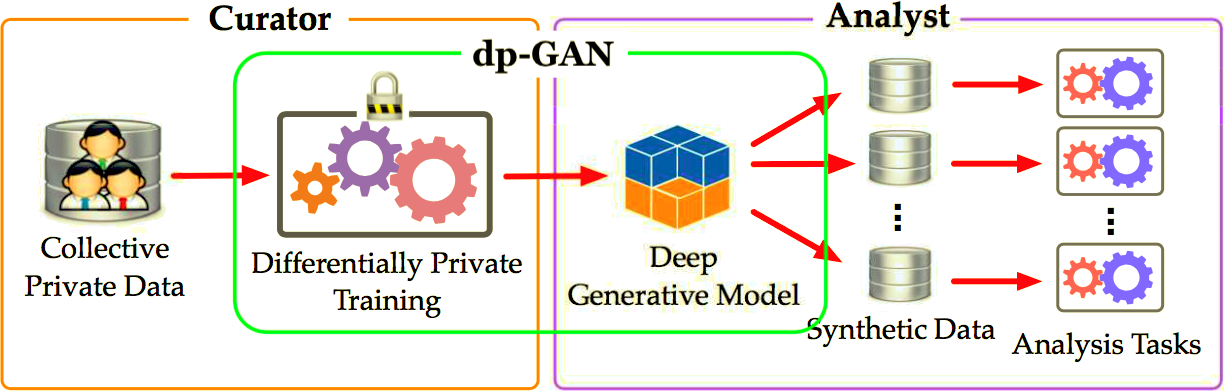
\includegraphics[width=0.7\textwidth]{dp-gan_role.png}
    \captionof{figure}{La place de dp-GAN dans la chaîne de traitement des données confidentielles. Le « \textit{curator} » est l'entité qui anonymise les données pour l'\textit{analyst}.}
    \label{dp-gan_role}
\end{figure}

\section{Implémentation}

\TODO{Un gros rapport, complet, avec explication du code, difficulté, est-ce que j'ai repris du début, mes résultats expérimentaux, etc.}

Cette section détaille mon implémentation de dp-GAN, les difficultés rencontrées et leurs solutions possibles --- implémentées ou non --- ainsi que les résultats obtenus.

Le code du projet est disponible sur Github à : \url{https://github.com/alexandrehuat/dp-gan}.

\subsection{Motivations}

Le véritable défi de ce projet, en accord avec l'objet du cours de \DL, est l'implémentation de dp-GAN basique. En effet, celle-ci demande une prise en main de WGAN amélioré et des calculs de confidentialité différentielle \citep{dlwdp, pinq}. En comparaison, dp-GAN avancé ne consiste qu'en l'enrichissement de dp-GAN basique d'un apprentissage sur des données publiques et d'un clustering hiérarchique des paramètres du réseau. Or, comptant ma formation en apprentissage statistique, ces opérations ne présentent pas de plus-value pédagogique. Sachant le temps allouable au projet, il m'est apparu raisonnable de me concentrer sur l'implémentation de dp-GAN basique. Quant aux données d'expérimentations, j'ai choisi d'utiliser MNIST pour faciliter l'apprentissage et l'interprétabilité des résultats.

\subsection{Technologie}

Dans \cite{dpgan}, les auteurs précisent avoir développé dp-GAN en TensorFlow. Étant donné l'avénement de TensorFlow dans la communauté du \DL

\subsection{Apprentissage}

préapprentissage
	AE 50 epochs, test mse = 0.0297
	CNN 2 epochs, test acc = 98.57 %

validation = 10 %

DIFFICULTÉS:
* première impl avec "with tf.Session()": app avec tf -> pred avec keras -> "FailedPreconditionError (see above for traceback): Attempting to use uninitialized value is_real/bias"
	solution: self.tf_session! référence jamais perdue donc calculs tjrs possible

\subsection{Test}

\printbibliography[title=Références,heading=bibintoc]

\end{document}

\begin{document}



\end{document}
\begin{document}



\end{document}
\begin{document}



\end{document}